\chapter{La historia del análisis real}

\section{Preámbulo}

\textbf{SIMPLICIO:} ¿Qué es el ``Análisis real''?

\textbf{SÓCRATES:} Oh, es simplemente Cálculo, pero hecho ``bien''.

\textbf{SIMPLICIO:} ¿Eh? ¿Por qué el Cálculo necesita un nombre nuevo?
¿Qué tiene de malo?

\textbf{SÓCRATES:} Bueno, nada en realidad. Rápido: ¿qué es una
derivada?

\textbf{SIMPLICIO:} ¡Fácil! Si tengo una función $f : \mathbb{R} \to \mathbb{R}$ y es
derivable en $x$, entonces la derivada es:
\[ f'(x) := \lim_{h \to 0} \frac{f(x+h)-f(x)}{h} \]
Esto representa la pendiente ``instantánea'' de la gráfica de la función
$y = f(x)$ en el punto $(x, f(x))$.

\begin{center}
    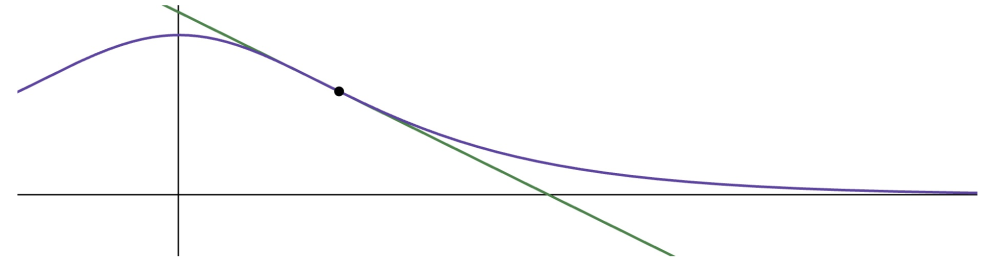
\includegraphics[width=0.5\linewidth]{fig/Derivada.png}
\end{center}

\textbf{SÓCRATES:} ¡Muy bien! Y dime por favor, ¿qué es una integral?

\textbf{SIMPLICIO:} ¡Eso también es fácil! Si quieres integrar nuestra
función $f$ a lo largo de un intervalo, $[a, b]$, por ejemplo, finges
que tienes infinitos rectángulos infinitamente pequeños, calculas sus
áreas como base por altura y los sumas:
\[ \int_{a}^{b} f(x)dx := \lim_{N \to \infty} \sum_{j=1}^{N} \frac{b-a}{N} f\left(a + j\frac{b-a}{N}\right) \]

\begin{center}
    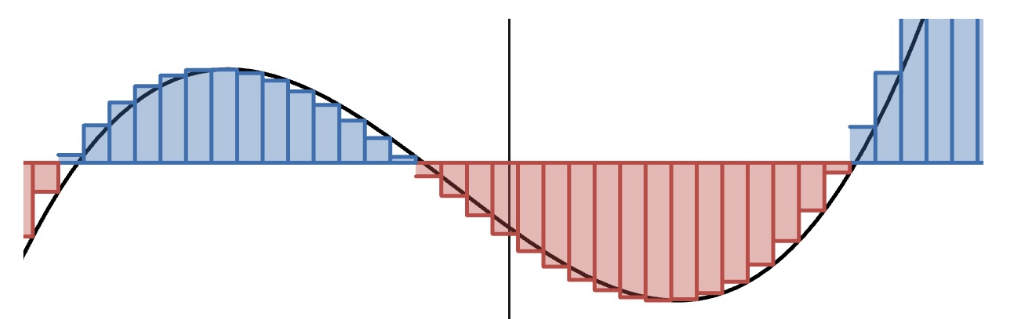
\includegraphics[width=0.5\linewidth]{fig/Integral.png}
\end{center}

\textbf{SÓCRATES:} Estupendo. ¿Y cuáles son los dos Teoremas
Fundamentales del Cálculo?

\textbf{SIMPLICIO:} ¡Estos también son fáciles! El primero dice que si
creas una nueva función integrando $f$ hasta una cantidad variable, $x$,
es decir, defines:
\[ F(x) := \int_{a}^{x} f(t)dt \]
entonces la derivada de la nueva función es simplemente $F'(x) = f(x)$.

\textbf{SÓCRATES:} ¿Y el segundo?

\textbf{SIMPLICIO:} El segundo dice que, a la inversa, si $F$ es una
primitiva de $f$, es decir, $F'(x) = f(x)$, entonces es fácil calcular
el área bajo la curva, porque:
\[ \int_{a}^{b} f(x)dx = F(b) - F(a) \]
¡Así que la derivación y la integración son operaciones inversas!

\textbf{SÓCRATES:} Perfecto. Ahora, aquí está el problema. Has usado
palabras como ``límite'', ``infinitos'', ``infinitamente pequeño'', y
así sucesivamente. ¿Qué significan \textit{realmente}?

\textbf{SIMPLICIO:} Oh, ya sabes, es cuando algo sucede
``eventualmente''. Solo tienes que acostumbrarte a la sensación.

\textbf{SÓCRATES:} Hmm sí, entiendo. Estoy de acuerdo en que esa es una
forma aceptable de pensarlo, al menos por un tiempo, y una que le iba
bien a Newton (que se sentía bastante incómodo con tales palabras) y a
Leibniz (que era más despreocupado en este aspecto), los dos inventores
del cálculo del siglo XVII (si no contamos a personas como los antiguos
griegos Eudoxo y Arquímedes, o al indio Madhava del siglo XIV... pero
esto no es una lección de historia). Leibniz enseñó a los hermanos
Bernoulli (¡los ``primeros estudiantes de bachillerato tecnológico'' del
mundo!), quienes enseñaron, entre otros, al marqués de l'Hôpital y al
gran Leonhard Euler (el primer ``nativo del cálculo''), quien nos enseñó
al resto de nosotros. Todo iba bastante bien... y entonces llegó el
siglo XIX.

\begin{center}
    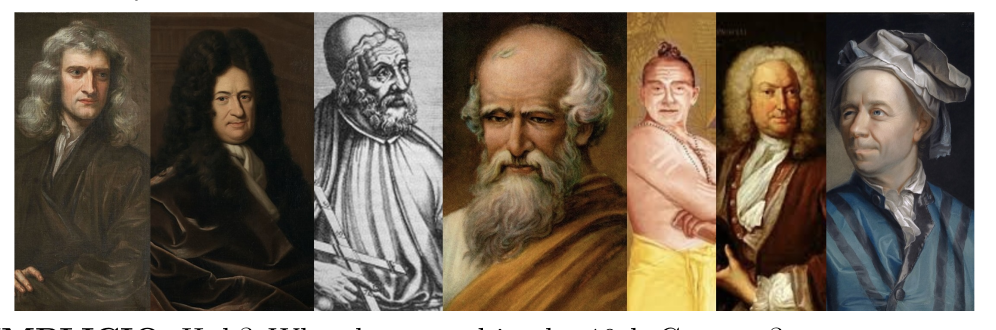
\includegraphics[width=0.5\linewidth]{fig/Matematicos.png}
\end{center}

\textbf{SIMPLICIO:} ¿Eh? ¿Qué pasó en el siglo XIX?

\textbf{SÓCRATES:} Verás, un tipo llamado Augustin-Louis Cauchy apareció
(más o menos en la década de 1810) y empezó a protestar porque no
estábamos haciendo las cosas de forma perfectamente ``rigurosa''. Se
propuso volver a demostrar los teoremas del cálculo usando definiciones
precisas en lugar de explicaciones vagas. Estaba haciendo grandes
progresos, incluyendo la demostración de afirmaciones como: el límite de
funciones continuas es continuo.

\begin{center}
    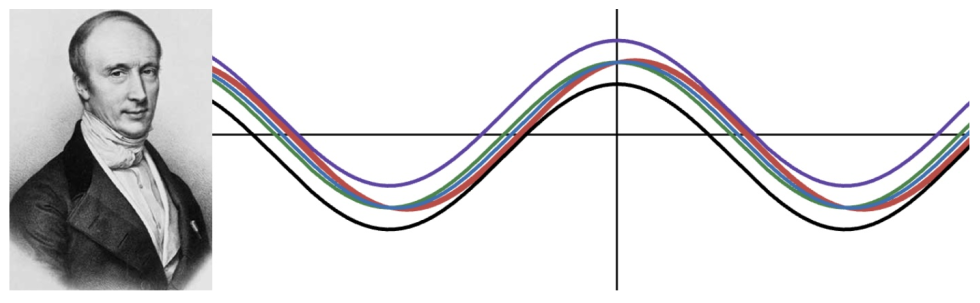
\includegraphics[width=0.5\linewidth]{fig/Cauchy.png}
\end{center}

\textbf{SIMPLICIO:} Claro, eso suena perfectamente razonable. Un límite
es un proceso continuo, así que si se lo aplicas a funciones continuas,
al final deberías obtener algo continuo también. ¿No?

\textbf{SÓCRATES:} Bueno, el problema es que por la misma época, un tipo
llamado Joseph Fourier andaba por ahí afirmando que podía sumar un
montón de senos y cosenos y obtener básicamente cualquier función que
quisiera, ¡incluyendo, por ejemplo, la función discontinua de diente de
sierra!

\textbf{SIMPLICIO:} ¡¿Qué?!

\textbf{SÓCRATES:} Mira tú mismo: aquí tienes una gráfica de
$\sum_{n=1}^{100} \frac{1}{n} \sin(nx)$. A medida que llevas el 100 al
infinito, ¡Fourier afirma que esto se acercará cada vez más a una
función de diente de sierra!

\begin{center}
    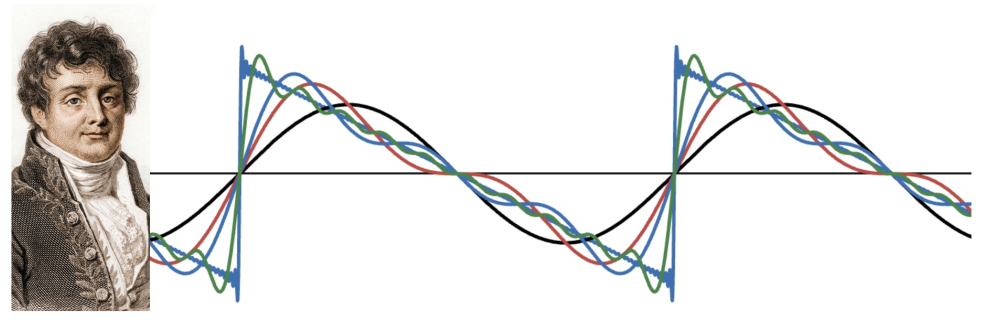
\includegraphics[width=0.5\linewidth]{fig/Fourier.png}
\end{center}

\textbf{SIMPLICIO:} ¡Hala! Espera, se me ocurre un ejemplo aún más
fácil: solo hay que mirar la familia más simple de polinomios, $f_n(x) =
x^n$, en el intervalo unidad $[0, 1]$. Cuando tomas potencias altas de
cualquier punto estrictamente menor que 1, eso tiende a 0 en el límite,
pero las potencias de 1 siempre se mantienen en 1. ¡Así que la función
límite también es discontinua! ¿Qué demonios está pasando aquí?

\begin{center}
    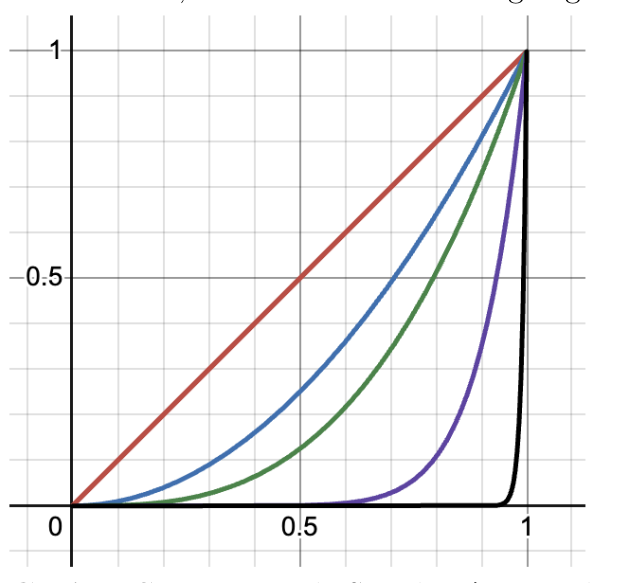
\includegraphics[width=0.5\linewidth]{fig/FamiliaDePolinomios.png}
\end{center}

\textbf{SÓCRATES:} ¡Muy bien, Simplicio! Exactamente, entre Fourier y
Cauchy, ``rompieron las matemáticas''. ¡El que lo rompe, lo paga!

\textbf{SIMPLICIO:} Vale, entonces ¿cuál es la respuesta correcta? ¿Cómo
se hace el cálculo con rigor?

\textbf{SÓCRATES:} ¡No tan rápido! Las cosas se pusieron aún peor, y a
mediados del siglo XIX, ¡la gente se dio cuenta de que ni siquiera
sabíamos qué \textit{son} los números reales!

\textbf{SIMPLICIO:} ¿Qué? ¿Cómo que qué son? Aquí los tienes: está el
cero, y el uno, y el $-2$, y $3/5$, y $\sqrt{2}$, y $e$ y $\pi$. ¿Cuál es
el problema?

\begin{center}
    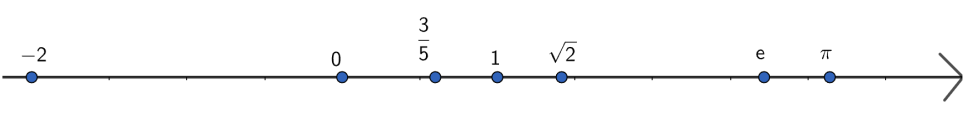
\includegraphics[width=0.5\linewidth]{fig/NumerosReales.png}
\end{center}

\textbf{SÓCRATES:} Bueno, ¿recuerdas que en cálculo necesitas algo
llamado el teorema del valor intermedio?

\textbf{SIMPLICIO:} Claro, si tienes una función continua y pasa de ser
negativa a ser positiva, entonces tiene que cruzar el cero en algún
punto intermedio.

\textbf{SÓCRATES:} Muy bien. Háblame de la función $f : x \mapsto x^2 -
2$. (Decimos: ``$f$ asigna $x$ a $x^2 - 2$''. Observa que escribimos $f
: \mathbb{R} \to \mathbb{R}$ para indicar que $f$ toma números reales y devuelve números
reales, pero sustituimos $\to$ por $\mapsto$ cuando queremos decir qué le ocurre
a una entrada particular $x$ bajo la acción de $f$). En particular, ¿qué
le ocurre a $f$ en los números racionales?

\textbf{SIMPLICIO:} Vale, bueno, si $x$ es un número racional, también
lo es $x^2$, y por tanto también $x^2 - 2$. Así que, en realidad,
podríamos decir que $f : \mathbb{Q} \to \mathbb{Q}$, es decir, $f$ asigna números racionales
a números racionales. Sobre los reales, la gráfica de $y = f(x)$ es una
parábola simple. Pero me habías preguntado por el teorema del valor
intermedio. Hmm. Cuando $x = 0$, sé que $f(0) = 0^2 - 2 = -2$, que es
negativo. Y cuando $x = 2$, $f(2) = 2^2 - 2 = 2$, que es positivo.

\textbf{SÓCRATES:} Continúa...

\textbf{SIMPLICIO:} Así que hay una raíz de $f$ en algún lugar entre 0 y
2. Pero el lugar donde $f$ cruza el eje $x$ es en $x = \sqrt{2} \approx 1.41
\dots$.

\textbf{SÓCRATES:} ¿And what did the Pythagoreans know about this number?

\textbf{SIMPLICIO:} Supuestamente uno de ellos, Hipaso, descubrió que
$\sqrt{2}$ es irracional, lo que arruinó toda su teoría de la geometría
y la forma (originalmente creían que \textit{todos} los números eran
racionales); la leyenda dice que Hipaso fue ahogado en el mar por su
herejía.

\textbf{SÓCRATES:} Entonces...

\textbf{SIMPLICIO:} ¡¿Entonces espera, si nos limitamos a las entradas
racionales, esta parábola es negativa, luego es positiva, y
\textit{nunca} cruza el cero?! Pero hay montones de números racionales
por todas partes. Entonces, ¿qué hace que los números reales sean
diferentes de los números racionales para que el Teorema del Valor
Intermedio sí se cumpla?

\textbf{SÓCRATES:} ¡Ah! Ahora, amigo mío, estamos listos para comenzar.

\section{Introducción a Lean}

\subsection*{Software de demostración de teoremas}

En este curso, utilizaremos un ``asistente de demostración'' llamado
Lean. Se trata de un software que comprueba que nuestras demostraciones
prueban \textit{exactamente} lo que afirmamos que prueban.

\begin{theorem}
Si sabemos que $x = 5$, entonces podemos demostrar que $x = 5$.
\end{theorem}

\begin{minted}{lean}
import Mathlib.Tactic

variable (x : ℝ)

-- 1ª demostración
example
  (h : x = 5)
  : x = 5 :=
by
  exact h

-- 2ª demostración
example
  (h : x = 5)
  : x = 5 :=
by
  apply h

-- 3ª demostración
example
  (h : x = 5)
  : x = 5 :=
by
  assumption
\end{minted}

\textbf{Nota:} Se escribe \texttt{exact h} ya que la hipótesis
\texttt{h} es exactamente lo que queremos demostrar.

\section{La táctica \texttt{rfl}}

\subsection*{Cuando las cosas son idénticas a sí mismas}

A veces, en matemáticas, necesitamos demostrar que algo es igual a sí
mismo. Por ejemplo, demostrar que $x^2 + 2y = x^2 + 2y$. En Lean, usamos
la táctica \texttt{rfl} (abreviatura de \textit{reflexivity}).

\begin{theorem}
Toda expresión matemática es igual a sí misma.
\end{theorem}

\begin{minted}{lean}
import Mathlib.Tactic

variable (x y : ℝ)

-- 1ª demostración
example : x ^ 2 + 2 * y = x ^ 2 + 2 * y :=
by
  rfl

-- 2ª demostración
example : x ^ 2 + 2 * y = x ^ 2 + 2 * y :=
by
  simp
\end{minted}

\section{La táctica \texttt{rw}}

\subsection*{Reescribir con igualdades}

Supongamos que tienes una hipótesis llamada \texttt{Bob : x = 2}, y tu
objetivo es demostrar que $x + y = 2 + y$. Como \texttt{Bob} nos dice
que $x = 2$, podemos sustituir $x$ por 2 usando \texttt{rewrite}.

\begin{theorem}
Si sabemos que $x = 2$, entonces podemos demostrar que $x + y = 2 + y$.
\end{theorem}

\begin{minted}{lean}
-- 1ª demostración
example
  (h : x = 2)
  : x + y = 2 + y :=
by
  rewrite [h]
  -- ⊢ 2 + y = 2 + y
  rfl

-- 2ª demostración
example
  (h : x = 2)
  : x + y = 2 + y :=
by
  subst h
  -- ⊢ 2 + y = 2 + y
  rfl

-- 3ª demostración
example
  (h : x = 2)
  : x + y = 2 + y :=
by
  rw [h]

-- 4ª demostración
example
  (h : x = 2)
  : x + y = 2 + y :=
by
  simp [h]
\end{minted}

\section{La táctica \texttt{ring\_nf}}

\subsection*{Manipulaciones algebraicas}

La táctica \texttt{ring\_nf} (ring normal form) puede realizar
automáticamente expansiones de productos, agrupar términos y aplicar la
propiedad distributiva.

\begin{theorem}
El desarrollo binomial: $(x + y)^3 = x^3 + 3x^2y + 3xy^2 + y^3$.
\end{theorem}

\begin{minted}{lean}
-- 1ª demostración
example : (x + y)^3 = x^3 + 3*x^2*y + 3*x*y^2 + y^3 :=
by
  ring

-- 2ª demostración
example : (x + y)^3 = x^3 + 3*x^2*y + 3*x*y^2 + y^3 :=
by
  ring_nf
\end{minted}

\section{La táctica \texttt{use}}

\subsection*{Demostrar la existencia}

Para demostrar una afirmación existencial ($\exists$), debes proporcionar un
valor específico que funcione usando la táctica \texttt{use}.

\begin{theorem}
  Existe un número real que hace que este desarrollo binomial funcione
  \[ (x + y)^4 = x^4 + 4*x^3*y + c*x^2*y^2 + 4*x*y^3 + y^4 \]
\end{theorem}

\begin{minted}{lean}
example : ∃ c, (x + y)^4 = x^4 + 4*x^3*y + c*x^2*y^2 + 4*x*y^3 + y^4 :=
by
  use 6
  -- ⊢ (x+y)^4 = x^4 + 4*x^3*y + 6*x^2*y^2 + 4*x*y^3 + y^4
  ring
\end{minted}

\section{La táctica \texttt{intro}}

\subsection*{Sentencias universales}

Para demostrar una afirmación ``para todo'' ($\forall$), introducimos un
elemento arbitrario y las hipótesis asociadas usando \texttt{intro}.

\begin{theorem}
Para todos los números reales positivos, se cumple esta identidad
algebraica.
\[(\epsilon + 1)^2 = (\epsilon + 1)^2 \]
\end{theorem}

\begin{minted}{lean}
example : ∀ ε : ℝ, ε > 0 → (ε + 1) ^ 2 = (ε + 1) ^ 2 :=
by
  intro ε h
  -- ε : ℝ
  -- h : ε > 0
  -- ⊢ (ε + 1) ^ 2 = (ε + 1) ^ 2
  rfl
\end{minted}

\section{La táctica \texttt{specialize}}

\subsection*{Uso de sentencias universales}

Si tienes un $\forall$ en una \textbf{hipótesis} y quieres aplicarlo a un
valor específico, usas \texttt{specialize}.

\begin{theorem}
Si una función de $x$ siempre es igual a $x^2$, entonces es igual a $t^2$ cuando se evalúa en $t$.
\end{theorem}

\begin{minted}{lean}
-- 1ª demostración
example
  (t : ℝ)
  (ht : t > 0)
  (f : ℝ → ℝ)
  (hf : ∀ x > 0, f x = x ^ 2)
  : f t = t ^ 2 :=
by
  specialize hf t
  -- hf : t > 0 → f t = t ^ 2
  specialize hf ht
  -- hf : f t = t ^ 2
  exact hf

-- 2ª demostración
example
  (t : ℝ)
  (ht : t > 0)
  (f : ℝ → ℝ)
  (hf : ∀ x > 0, f x = x ^ 2)
  : f t = t ^ 2 :=
by
  apply hf
  -- ⊢ t > 0
  exact ht

-- 3ª demostración
-- ===============

example
  (t : ℝ)
  (ht : t > 0)
  (f : ℝ → ℝ)
  (hf : ∀ x > 0, f x = x ^ 2)
  : f t = t ^ 2 :=
by
  exact hf t ht

-- 4ª demostración
-- ===============

example
  (t : ℝ)
  (ht : t > 0)
  (f : ℝ → ℝ)
  (hf : ∀ x > 0, f x = x ^ 2)
  : f t = t ^ 2 :=
by
  rw [hf]
  -- ⊢ t > 0
  exact ht

-- 5ª demostración
-- ===============

example
  (t : ℝ)
  (ht : t > 0)
  (f : ℝ → ℝ)
  (hf : ∀ x > 0, f x = x ^ 2)
  : f t = t ^ 2 :=
by
  simp_all

-- 6ª demostración
-- ===============

example
  (t : ℝ)
  (ht : t > 0)
  (f : ℝ → ℝ)
  (hf : ∀ x > 0, f x = x ^ 2)
  : f t = t ^ 2 :=
by
  aesop

-- 7ª demostración
-- ===============

example
  (t : ℝ)
  (ht : t > 0)
  (f : ℝ → ℝ)
  (hf : ∀ x > 0, f x = x ^ 2)
  : f t = t ^ 2 :=
by
  solve_by_elim
\end{minted}

\section{El desafío táctico definitivo}

\subsection*{El desafío final}
Aquí tienes la ``Hoja de trucos de los cuantificadores'':

\begin{center}
\begin{tabular}{|l|c|c|}
\hline
Empieza con: & $\forall$ & $\exists$ \\ \hline
\textbf{Objetivo}  & \texttt{intro}      & \texttt{use} \\ \hline
\textbf{Hipótesis} & \texttt{specialize} & \texttt{choose} \\ \hline
\end{tabular}
\end{center}

\begin{theorem}
Dada una función con propiedades específicas, podemos demostrar una
afirmación compleja que implica existencia y universales.
\end{theorem}

\begin{minted}{lean}
-- 1ª demostración
example
  (f : ℝ → ℝ)
  (h1 : ∃ a : ℝ, f a = 3)
  (h2 : ∀ x > 0, f (x + 1) = f x + 9)
  : ∃ b : ℝ, ∀ y > 0, f (y + 1) ^ 2 = (f y + (f b) ^ 2) ^ 2 :=
by
  choose a ha using h1
  -- a : ℝ
  -- ha : f a = 3
  use a
  -- ⊢ ∀ y > 0, f (y + 1) ^ 2 = (f y + f a ^ 2) ^ 2
  intro y hy
  -- y : ℝ
  -- hy : y > 0
  -- ⊢ f (y + 1) ^ 2 = (f y + f a ^ 2) ^ 2
  specialize h2 y hy
  -- h2 : f (y + 1) = f y + 9
  rewrite [h2]
  -- ⊢ (f y + 9) ^ 2 = (f y + f a ^ 2) ^ 2
  rewrite [ha]
  -- ⊢ (f y + 9) ^ 2 = (f y + 3 ^ 2) ^ 2
  ring_nf

-- 2ª demostración
example
  (f : ℝ → ℝ)
  (h1 : ∃ a : ℝ, f a = 3)
  (h2 : ∀ x > 0, f (x + 1) = f x + 9)
  : ∃ b : ℝ, ∀ y > 0, f (y + 1) ^ 2 = (f y + (f b) ^ 2) ^ 2 :=
by
  obtain ⟨a, ha⟩ := h1
  -- a : ℝ
  -- ha : f a = 3
  use a
  -- ⊢ ∀ y > 0, f (y + 1) ^ 2 = (f y + f a ^ 2) ^ 2
  intro y hy
  -- y : ℝ
  -- hy : y > 0
  -- ⊢ f (y + 1) ^ 2 = (f y + f a ^ 2) ^ 2
  rw [h2 y hy]
  -- ⊢ (f y + 9) ^ 2 = (f y + f a ^ 2) ^ 2
  rw [ha]
  -- ⊢ (f y + 9) ^ 2 = (f y + 3 ^ 2) ^ 2
  norm_num

-- 3ª demostración
example
  (f : ℝ → ℝ)
  (h1 : ∃ a : ℝ, f a = 3)
  (h2 : ∀ x > 0, f (x + 1) = f x + 9)
  : ∃ b : ℝ, ∀ y > 0, f (y + 1) ^ 2 = (f y + (f b) ^ 2) ^ 2 :=
by
  obtain ⟨a, ha⟩ := h1
  -- a : ℝ
  -- ha : f a = 3
  use a
  -- ⊢ ∀ y > 0, f (y + 1) ^ 2 = (f y + f a ^ 2) ^ 2
  grind

-- 4ª demostración
example
  (f : ℝ → ℝ)
  (h1 : ∃ a : ℝ, f a = 3)
  (h2 : ∀ x > 0, f (x + 1) = f x + 9)
  : ∃ b : ℝ, ∀ y > 0, f (y + 1) ^ 2 = (f y + (f b) ^ 2) ^ 2 :=
by
  rcases h1 with ⟨a, ha⟩
  -- a : ℝ
  -- ha : f a = 3
  use a
  -- ⊢ ∀ y > 0, f (y + 1) ^ 2 = (f y + f a ^ 2) ^ 2
  grind
\end{minted}

\section*{Epílogo}

¡Victoria! Has completado un argumento matemático genuinamente
sofisticado. Usar un demostrador de teoremas es como aprender ajedrez:
es mucho más fácil ver el tablero que leer solo la notación. Esta
retroalimentación inmediata construye la intuición necesaria para el
cálculo riguroso.

%%% Local Variables:
%%% mode: latex
%%% TeX-master: "Analisis_en_Lean"
%%% End:
